\documentclass[10pt]{beamer}

\usepackage[utf8]{inputenc}
\usepackage[T1]{fontenc}
\usepackage{textcomp}
\usepackage[french]{babel}
\usepackage{amsmath, amssymb}
\usepackage{multicol}
\usepackage{mathtools}
\usepackage{graphicx}
\usepackage[inline]{asymptote}
\usepackage{tikz}

\usefonttheme{serif}

%\definecolor{white}{HTML}{faf4ed}
\definecolor{black}{HTML}{575279}
\definecolor{mauve}{HTML}{907aa9}
\definecolor{blue}{HTML}{286983}
\definecolor{red}{HTML}{d7827e}
\definecolor{yellow}{HTML}{ea9d34}
\definecolor{gray}{HTML}{9893a5}
\definecolor{grey}{HTML}{9893a5}

\definecolor{sirred}{HTML}{EF9A9A}
\definecolor{sirpurple}{HTML}{E1BEE7}
\definecolor{sirgreen}{HTML}{C5E1A5}
\definecolor{sircyan}{HTML}{80DEEA}

%\pagecolor{white}
\color{black}

%\renewcommand{\familydefault}{\rmdefault}
\setbeamertemplate{navigation symbols}{}

\newcommand{\cir}[1]{\tikz \draw[black, fill=sir#1] (0,0) circle (3pt);}

\let\ds\displaystyle

\begin{document}
	% Intro
	\begin{frame}
		\begin{center}
			\vfill

			{\large Comment la structure de la ville affecte les inégalités comportementales face à une épidémie ?}

			\vfill
			\vfill

			{\footnotesize Hugo {\sc Salou}}\\
			{\it\scriptsize MP2I}
		\end{center}
	\end{frame}

	% Lien avec le thème
	\begin{frame}
		\begin{itemize}
			\item 2 dernières années $\to$ pandémie
			\item importance de la structure de la ville
		\end{itemize}
	\end{frame}

	% Modèle SIR
	\begin{frame}
		\centering{\large Modèle SIR}

		\[
			\begin{array}{crl}
				\cir{cyan}&S&\longrightarrow~\text{Saines}\\
				\cir{red}&I&\longrightarrow~\text{Infectées}\\
				\cir{green}&R&\longrightarrow~\text{Rétablies}\\
				\cir{purple}&D&\longrightarrow~\text{Décédées}\\
			\end{array}\qquad
			\scalebox{0.8}{$\begin{array}{l}
				\ds\frac{\mathrm{d}S}{\mathrm{d}t}(t) = -r\,S(t)\,I(t)\\[5mm]
				\ds\frac{\mathrm{d}I}{\mathrm{d}t}(t) = r\,S(t)\,I(t) - (a+b)\,I(t)\\[5mm]
				\ds\frac{\mathrm{d}R}{\mathrm{d}t}(t) = a\,I(t)\\[5mm]
				\ds\frac{\mathrm{d}D}{\mathrm{d}t}(t) = b\,I(t)\\
			\end{array}$}
		\]

		\begin{figure}[H]
			\centering
			
\includegraphics{figure-sir.eps}
		\end{figure}
	\end{frame}

	% Modèle automate cellulaire
	\begin{frame}
		\centering{\large Modèle Automate cellulaire}

		\begin{multicols}{3}
			\begin{figure}[H]
				\centering
				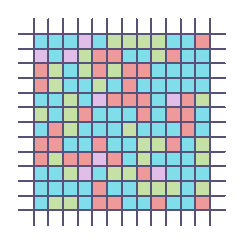
\includegraphics{figure-cellular-automaton.eps}
			\end{figure}
			\begin{figure}[H]
				\centering
				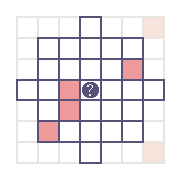
\includegraphics{figure-cellular-automaton-infect.eps}
			\end{figure}
			$\begin{array}{rcl}
				\cir{cyan}&\longrightarrow&\cir{cyan} \text{ ou } \cir{red}\\
				\cir{red}&\longrightarrow&\cir{red},\:\cir{green} \text{ ou } \cir{purple}\\
				\cir{purple}&\longrightarrow&\cir{purple}\\
				\cir{green}&\longrightarrow&\cir{green}
			\end{array}$
		\end{multicols}
		\begin{figure}[H]
			\centering
			
\includegraphics{figure-cellular-automaton-curve.eps}
		\end{figure}
	\end{frame}

	\begin{frame}
		\centering{\large Modèle particulaire}

		\begin{multicols}{2}
			\begin{figure}[H]
				\centering
				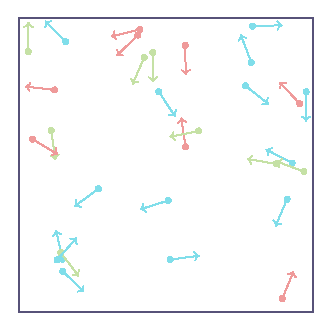
\includegraphics{figure-gas.eps}
			\end{figure}
			\begin{figure}[H]
				\centering
				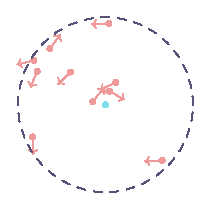
\includegraphics{figure-gas-near.eps}
			\end{figure}
		\end{multicols}
	\end{frame}

	\begin{frame}
	\end{frame}
\end{document}
